% update for ECCV'14 by Michael Stark and Mario Fritz
% updated in April 2002 by Antje Endemann
% Based on CVPR 07 and LNCS, with modifications by DAF, AZ and elle, 2008 and AA, 2010, and CC, 2011; TT, 2014

\documentclass[runningheads]{llncs}
\usepackage{graphicx}
\usepackage{amsmath,amssymb} % define this before the line numbering.
\usepackage{color}
\usepackage[width=122mm,left=12mm,paperwidth=146mm,height=193mm,top=12mm,paperheight=217mm]{geometry}
%\usepackage{ruler}
\usepackage{array}
\usepackage{float}
\usepackage{subfig,caption}
\usepackage{lipsum}
\usepackage{comment}
\usepackage{epstopdf}
%\usepackage{tablefootnote}
\renewcommand{\arraystretch}{1.1}

\newcommand{\todo}[1]{{\color{red} {\bf TODO:} \it #1}}
\begin{document}
% \renewcommand\thelinenumber{\color[rgb]{0.2,0.5,0.8}\normalfont\sffamily\scriptsize\arabic{linenumber}\color[rgb]{0,0,0}}
% \renewcommand\makeLineNumber {\hss\thelinenumber\ \hspace{6mm} \rlap{\hskip\textwidth\ \hspace{6.5mm}\thelinenumber}}
% \linenumbers
\pagestyle{headings}
\mainmatter
\title{Analyzing the Performance of Multilayer Neural Networks for Object Recognition}
% Replace with your title

\titlerunning{Analyzing The Performance of Multilayer Neural Networks}


\authorrunning{Pulkit Agrawal, Ross Girshick, Jitendra Malik}

\author{Pulkit Agrawal, Ross Girshick, Jitendra Malik \\ \texttt{\{pulkitag,rbg,malik\}@eecs.berkeley.edu}}
\institute{University of California Berkeley}


\maketitle
\begin{center}
\large{Supplementary Material} 
\end{center}
\section{Effect of fine-tuning on CNN parameters}
In the main paper we have provided additional evidence that fine-tuning a discriminatively pre-trained network is very effective in terms of task performance.
We also provided insights into how fine-tuning changes its parameters.
Here we describe this procedure in more detail and discuss alternative metrics for determining the effect of fine-tuning.
%\subsection{Effect of fine-tuning on network parameters}
\subsection{Defining the measure of discriminative capacity of a filter}
\label{sub:fine-entropy}
%We have provided additional evidence that fine-tuning a discriminatively pre-trained network is very effective in terms of task performance.
%Now we look inside the network to see how fine-tuning changes its parameters.
%To do this, we define a way to measure the capacity of each filter in the network to discriminate between object classes.

To measure the discriminative capacity of a filter, we start by collecting filter responses from a set of $N$ images.
Each image, when passed through the CNN produces a $p \times p$ heat map of scores for each filter in a given layer (e.g., $p = 6$ for a conv-5 filter and $p = 1$ for an fc-6 filter).
This heat map is vectorized (\texttt{x(:)} in MATLAB) into a vector of scores of length $p^2$. With each element of this vector we associate the class label of the image. 
Thus, for every image we have a score vector and a label vector of length $p^2$ each.
Next, the score vectors from all $N$ images are concatenated into an $Np^2$-length score vector.
The same is done for the label vectors.

Now, for a given score threshold $\tau$, we define the \emph{class entropy of a filter} to be the entropy of the normalized histogram of class labels that have an associated score $\geq \tau$.
A low class entropy means that at scores above $\tau$, the filter is very class selective.
As this threshold changes, the class entropy traces out a curve which we call the \emph{entropy curve}.
The \emph{area under the entropy curve} (AuE), summarizes the class entropy at all thresholds and is used as a measure of discriminative capacity of the filter. 
The lower the AuE value, the more class selective the filter is.

We can also characterize the distribution of discriminative ability of all filters of a layer.
To do this, we sort the filter according to their AuE.
Then, the cumulative sum of AuE values in the sorted list is calculated (called \emph{cumulative AuE} or CAuE). 
The $i$-th entry of the CAuE list is the sum of the AuE scores of the top $i$ most discriminative filters.
The difference in the value of the $i$-th entry before and after fine-tuning measures the change in class selectivity of the top $i$ most discriminative filters due to fine-tuning.
For comparing results across different layers, the CAuE values are normalized to account for different numbers of filters in each layer. 
Specifically, the $i$-th entry of the CAuE list is divided by $i$. 
This normalized CAuE is called the Mean Cumulative Area Under the Entropy Curve (MCAuE).
A lower value of MCAuE indicates that the set filters is more discriminative.

%Figure \ref{fig:fine-entropy} shows MCAuE computed on PASCAL-DET-GT image-label pairs using two networks: the first, was pre-trained on ImageNet only whereas the second was fine-tuned for PASCAL-DET. 
%The  $k^{th}$ threshold point for layer l corresponds to MCAuE of top $N_l(k/30)$ filters, where $N_l$ is number of filters in layer $l$. 
%PASCAL-DET-GT was used for this study instead of classification to ensure that filter responses were a direct result of presence of object categories of interest and not the background as might happen in the classification task.


\subsection{Defining the measure of discriminative capacity of a filter}
\label{sub:fine-entropy}
To measure the discriminative capacity of a filter, we start by collecting filter responses from a set of $N$ images.
Each image, when passed through the CNN produces a $p \times p$ heat map of scores for each filter in a given layer (e.g., $p = 6$ for a conv-5 filter and $p = 1$ for an fc-6 filter).
This heat map is vectorized (\texttt{x(:)} in MATLAB) into a vector of scores of length $p^2$. With each element of this vector we associate the class label of the image. 
Thus, for every image we have a score vector and a label vector of length $p^2$ each.
Next, the score vectors from all $N$ images are concatenated into an $Np^2$-length score vector.
The same is done for the label vectors.

Now, for a given score threshold $\tau$, we define the \emph{class entropy of a filter} to be the entropy of the normalized histogram of class labels that have an associated score $\geq \tau$.
A low class entropy means that at scores above $\tau$, the filter is very class selective.
As this threshold changes, the class entropy traces out a curve which we call the \emph{entropy curve}.
The \emph{area under the entropy curve} (AuE), summarizes the class entropy at all thresholds and is used as a measure of discriminative capacity of the filter. 
The lower the AuE value, the more class selective the filter is.

\subsection{Defining discriminative capacity of a layer}
We discuss three slightly different ways of defining the discriminative capacity of a layer. 

\subsubsection{Label Entropy}
\label{sub:def-label-ent}
The discriminative capacity of layer is computed as following: We sort the filter according to their AuE.
Then, the cumulative sum of AuE values in the sorted list is calculated (called \emph{cumulative AuE} or CAuE). 
The $i$-th entry of the CAuE list is the sum of the AuE scores of the top $i$ most discriminative filters.
The difference in the value of the $i$-th entry before and after fine-tuning measures the change in class selectivity of the top $i$ most discriminative filters due to fine-tuning.
For comparing results across different layers, the CAuE values are normalized to account for different numbers of filters in each layer. 
Specifically, the $i$-th entry of the CAuE list is divided by $i$. 
This normalized CAuE is called the Mean Cumulative Area Under the Entropy Curve (MCAuE).
A lower value of MCAuE indicates that the set filters is more discriminative.

\subsubsection{Weighted Label Entropy}
\label{sub:def-weighted-label-ent}
When computing the label histogram for computing AuE, instead of the label count we use the sum of the scores associated with the labels to construct the histogram. (Note: Since we are using outputs from relu or rectified linear units, all scores are $\geq 0$.)

\subsubsection{Spatial-Max (spMax) Label Entropy}
\label{sub:def-spmax-label-ent}
From the heatmap, we chose the element which has the maximum value and associate with it the label of the image class. Thus, for each image we have a score vector and a label vector of length $1$ each. Next, we concatenate score vectors and label vectors from N images into a  score vector and a  label vector  of size $N$ each. Now for every score threshold $(t)$ we consider all the labels which have an associated score $\geq t$. Next, we compute the entropy as in the case of Label-Entropy.

\setlength{\tabcolsep}{1pt}
\begin{table}
\begin{center}
\caption{This table lists percentage decrease in MCAuE as a result of finetuning when only 0.1, 0.25, 0.50 and 1.00 fraction of all the filters were used for computing MCAuE. A lower MCAuE indicates that filters in a layer are more selective/class specific. The 0.1 fraction includes the top 10\% most selective filters, 0.25 is top 25\% of most selective filters. Consequently, comparing MCAuE at different fraction of filters gives a better sense of how selective the ``most" selective filters have become to how selective all the filters have become.
A negative value in the tabel below indicates increase in entropy. Note that for all the metrics maximum decrease in entropy takes place while moving from layer 5 to layer 7. Also, note that for relu-6 and relu-7 the values in Label-Entropy and spMax-Label-Entropy are same as relu-6 and 7 have spatial maps of size 1.}
\label{table:fine-change}
\scalebox{0.85}{
\newcolumntype{d}[2]{D{.}{\cdot}{#1} }
\begin{tabular}{|c|p{1cm} p{1cm} p{1cm} p{1cm}| p{1cm} p{1cm} p{1cm} p{1cm}|p{1cm} p{1cm} p{1cm} p{1cm}|}
\hline
Layer & \multicolumn{4}{c|}{Label-Entropy} & \multicolumn{4}{c|}{Weighted-Label-Entropy} & \multicolumn{4}{c|}{spMax-Label-Entropy} \\
\hline
& 0.1 & 0.25 & 0.5 & 1.0 & 0.1 & 0.25 & 0.5 & 1 & 0.1 & 0.25 & 0.5 & 1.0 \\
\hline
pool-1 & $-0.02$  & $-0.14 $  & $-0.19$  & $-0.19$  & $0.06$  & $-0.13$  & $-0.16$  & $-0.16$  & $0.19$  & $0.10$  & $0.07$  & $0.04$   \\
pool-2 & $-0.71$  & $-0.31$   & $-0.14$  & $0.01$  & $0.41$  & $0.53$  & $0.58$  & $0.57$  & $-0.39$  & $-0.03$  & $0.11$  & $0.23$  \\ 
relu-3 & $-1.14$  & $-0.86$   & $-0.67$  & $-0.44$ & $1.11$  & $0.66$  & $0.52$  & $0.32$ & $0.14$  & $0.20$  & $0.32$  & $0.33$   \\
relu-4 & $-0.54$  & $-0.31$  & $-0.19$  & $-0.05$ & $-0.10$  & $0.55$  & $0.64$  & $0.57$  & $0.93$  & $0.97$  & $0.80$  & $0.65$ \\
pool-5 & $0.97$  & $0.55$  & $0.43$  & $0.36$ & $5.84$  & $3.53$  & $2.66$  & $1.85$  & $4.87$  & $3.05$  & $2.31$  & $1.62$   \\
relu-6 & $6.52$  & $5.06$  & $3.92$  & $2.64$  & $9.59$  & $7.55$  & $6.08$  & $4.27$ & $6.52$  & $5.06$  & $3.92$  & $2.64$   \\
relu-7 & $5.17$  & $2.66$  & $1.33$  & $0.44$  & $20.58$  & $14.75$  & $11.12$  & $7.78$  & $5.17$  & $2.66$  & $1.33$  & $0.44$  \\
\hline
\end{tabular}}
\end{center}
\end{table}
\setlength{\tabcolsep}{1.4pt}

\begin{figure}
\centering
\subfloat{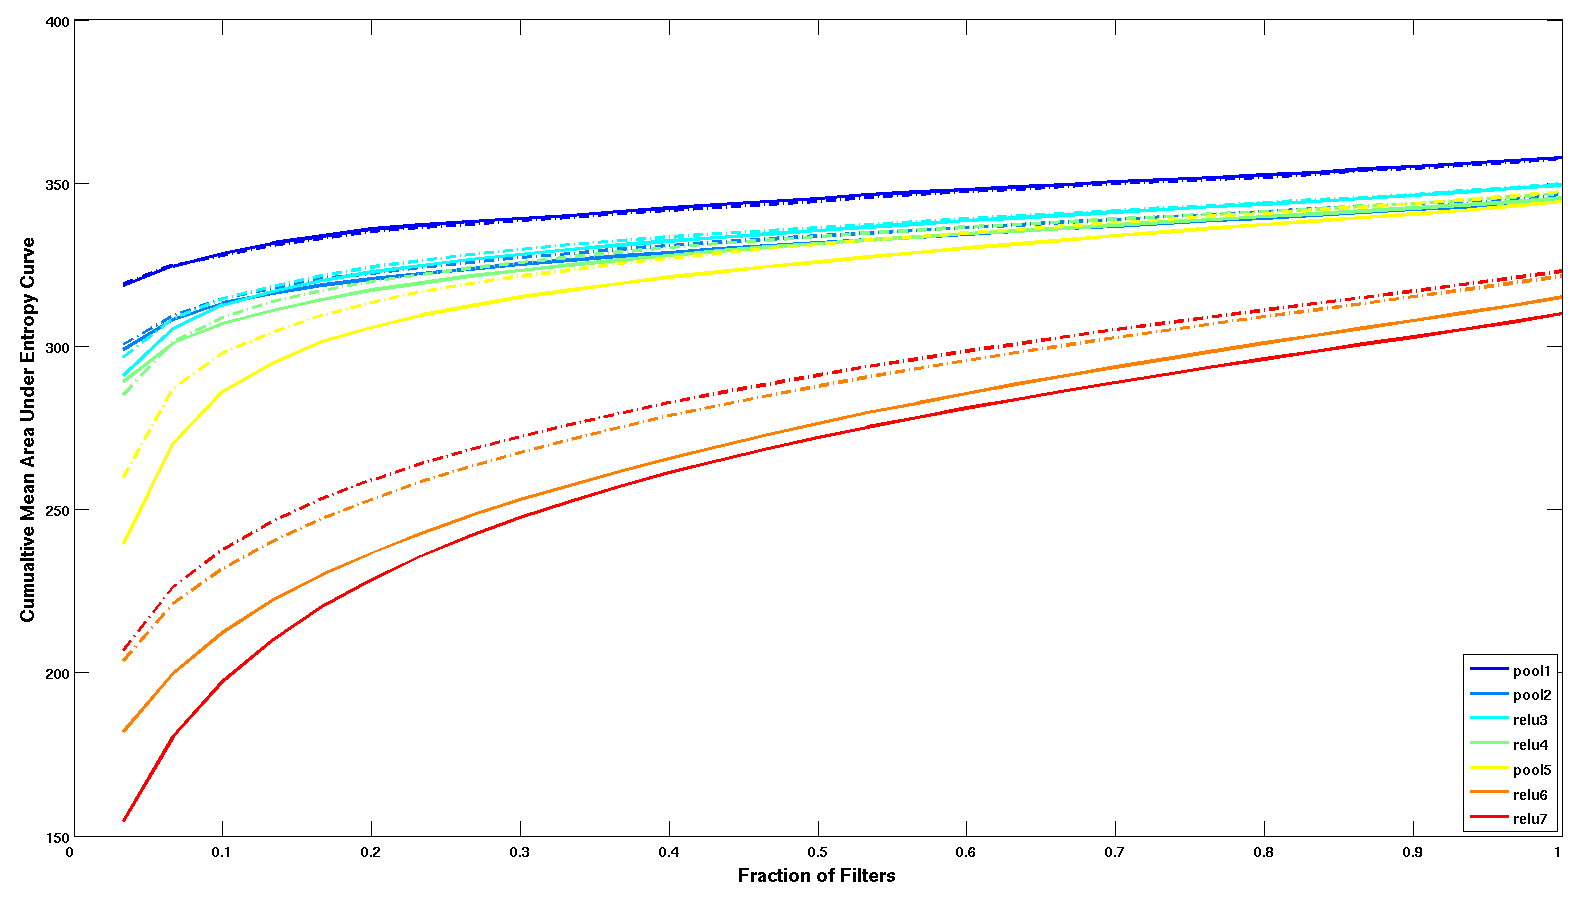
\includegraphics[scale=0.15]{images/weighted_layer_entropy.png}} \\
\subfloat{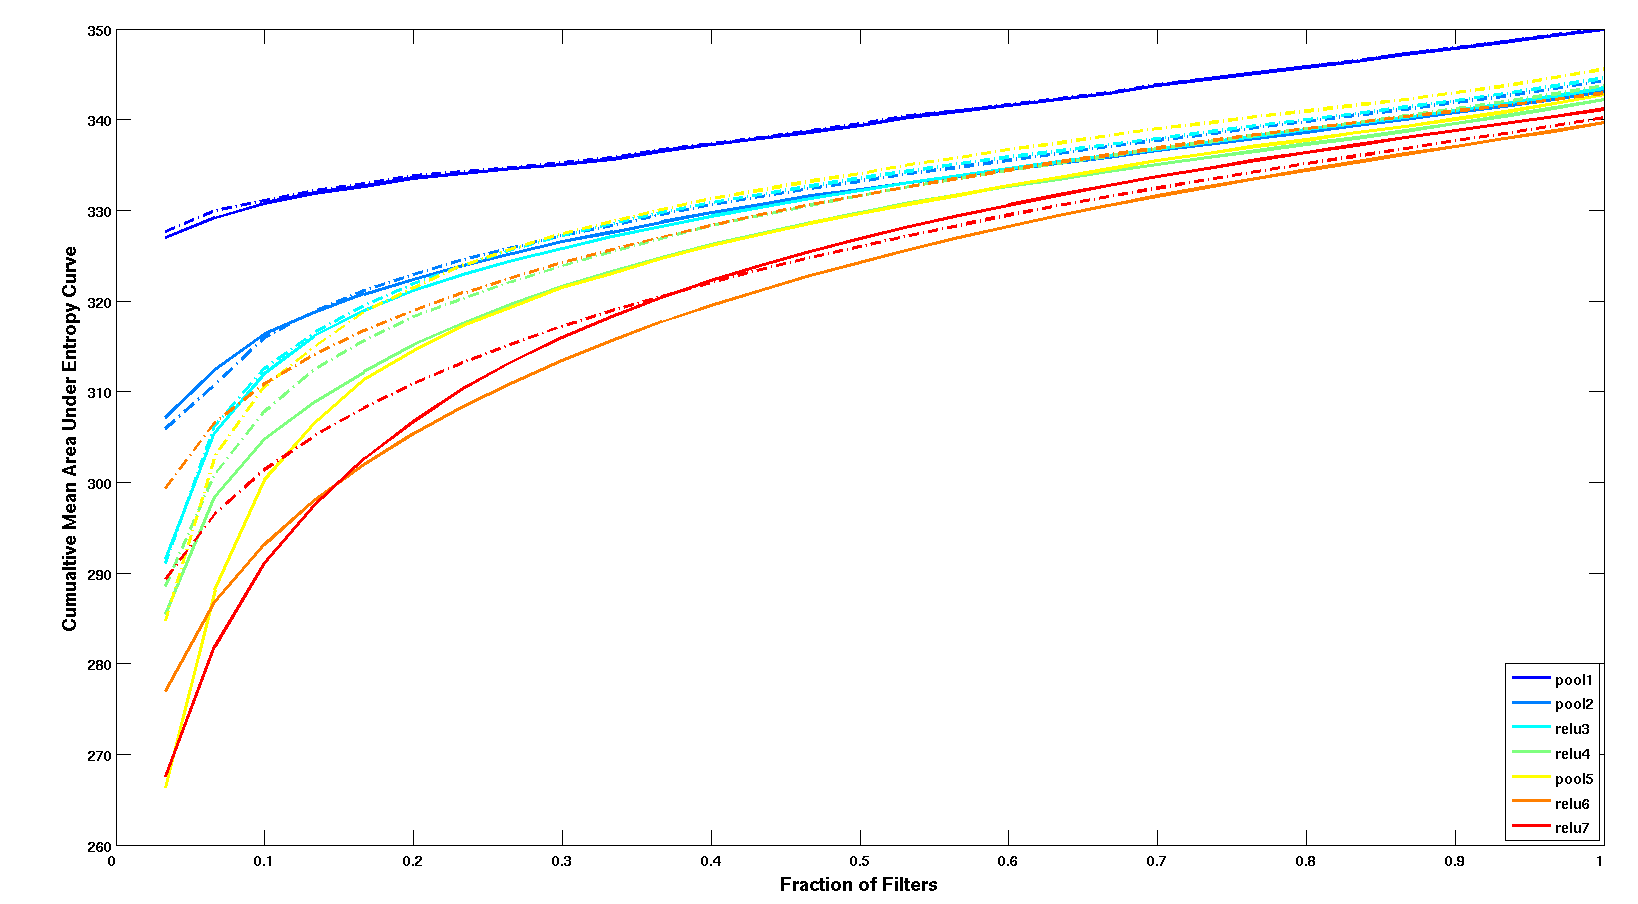
\includegraphics[scale=0.15]{images/spmax_layer_entropy.png}}
\caption{Mean Cumulative AuE plotted as fraction of filters for all layers of the Conv-Net. Dash-Dot Line: Alex-Net, Solid Line: Fine-Tuned Network. The top plot shows entropy calculated using Weighted-Label-Entropy Method, whereas the bottom plot entropy calculated using spMax-Label-Entropy Method. (see sec \ref{sub:def-label-ent} for method definitions.)}
\label{fig:fine-entropy}
\end{figure}

\subsection{Discussion}
The change in MCAuE for different layers as measured using alternative definitions of entropy can be seen in fig \ref{fig:fine-entropy} (Please see sec 3 of the main paper for more details on the procedure). A quantitative measure of change in entropy after finetuning is provided in table \ref{table:fine-change}. The percentage change in MCAuE is calculated as:
\begin{eqnarray}
\text{Percent Decrease} = 100 \times \frac{MCAuE_{untuned} - MCAuE_{fine}}{MCAuE_{untuned}}
\end{eqnarray}
where, $MCAuE_{fine}$ is for fine-tuned network and $MCAuE_{untuned}$ is for network trained on imagenet only.

Although, the most natural way to compute entropy is Label-Entropy as used by \cite{Breiman}, \cite{AmitGeman}, the alternative metrics also support the claim that most of the changes due to fine-tuning happen while moving from layers 5 to 7. At the same time, it is noteworthy, that for label-entropy pool-5 undergoes negligible change in entropy, whereas changes in pool-5 as measured by Weighted-Label Entropy and spMax-Label-Entropy are comparable to changes in relu-6 and relu-7.





%\section{Conclusion}
%\label{sec:conclusion}
%In this paper we analysed different properties of convolutional neural networks with the aim of gaining insights required to efficiently exploit the rich feature hierarchies provided by such networks. \\



\bibliographystyle{splncs03}
\bibliography{egbib}
\end{document}
